\chapter{Theoretical Background and Notation}\label{sec:theory}

\section{Kinematics}\label{sec:kinematics}
This section gives a compact overview about the notation for the kinematic and dynamic representation.  Each part is accompanied by some code snippets that should highlight how this works in Matlab.  Note: these code parts DO NOT belong to a specific example.  For complete examples check \secref{sec:ex}.

\subsection{Generalized Coordinates}
We use generalized coordinates $\mathbf{q}$ that can contain in the case of free floating bodies in addition to the joint coordinates $\mathbf{q}_{r}$ also un-actuated base coordinates $\mathbf{q}_b$: 
\begin{equation}
\mathbf{q} = \left( \begin{array}{c} \mathbf{q}_{b} \\ \mathbf{q}_{r} \end{array}\right).
\end{equation}

\begin{lstlisting}
% define generalized coordinates 
syms x q1 q2 real
q = [x,q1,q2]';
% define generalized velocities
syms Dx Dq1 Dq2 real
dq = [Dx,Dq1,Dq2]';
\end{lstlisting}

\subsection{Position Vector}
A (position) vector from point $O$ to $P$ as a function of generalized coordinates $\mathbf{q}$ expressed in frame $B$:
\begin{equation}
_B \mathbf{r}_{OP} = _B \mathbf{r}_{OP}\left(\mathbf{q}\right).
\end{equation}
\begin{lstlisting}
% define certain parameters
syms l real
% position vector
r = [l*sin(q1),l*cos(q1),0];
\end{lstlisting}


\subsection{Velocity (in Moved Systems)}\label{sec:velocity}
The velocity is given through differentiation, whereby special attention is required when differentiating in a moving (with respect to inertial frame $I$) coordinates system $B$:
\begin{eqnarray}
_I\mathbf{r} \rightarrow {}_I\dot{\mathbf{r}} &=& \frac{d{}_I\mathbf{r}}{dt} \\
_B\mathbf{r} \rightarrow {}_B\dot{\mathbf{r}} &=& \frac{d{}_B\mathbf{r}}{dt} + _B\omega_{IB} \times _B\mathbf{r}
\end{eqnarray}
In this document, $O$ refers to the origin of a frame, $I$ indicates the inertial frame and $B$ a body fixed frame (which can be moved).
\\

%In the special case of rigid body kinematics we introduce the body rotation speed $\boldsymbol{\Omega}$
%\begin{equation}
%\boldsymbol{\Omega} = {}_I\omega_{IB}
%\end{equation}


\begin{lstlisting}
% derivation of position vectors expressed in inertia frame
dr = dMATdt(r,q,dq);
\end{lstlisting}

\subsection{Rotation}
\begin{figure}[H]
	\centering
		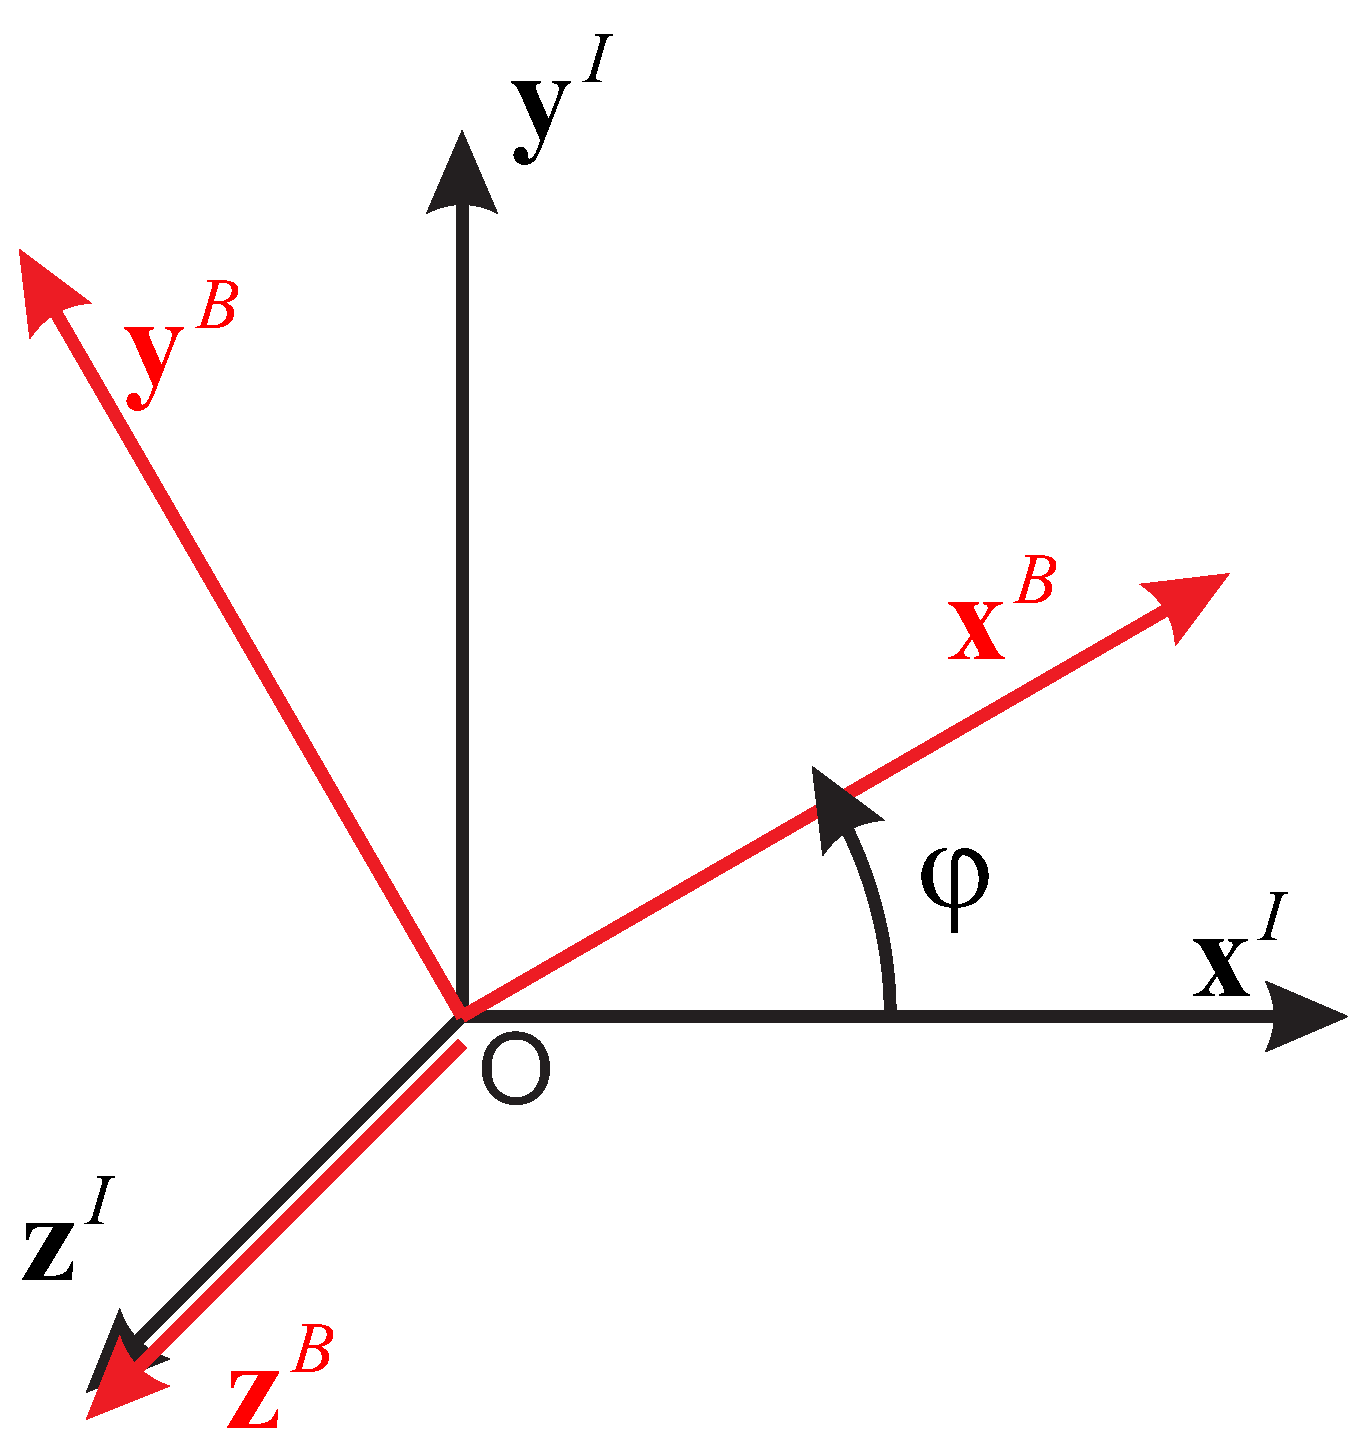
\includegraphics[width=.500\textwidth]{pics/movedCS.pdf}
	\caption{Rotated coordinate system $B$ around z axis}
	\label{fig:movedCS}
\end{figure}

The rotation matrix $\mathbf{A}_{IB}$ rotates a vector $_B\mathbf{r}$ expressed in frame $B$ to frame $I$:
\begin{eqnarray}
_I\mathbf{r} &=& \mathbf{A}_{IB} {}_B\mathbf{r}\\
_B\mathbf{r} &=& \mathbf{A}_{BI} {}_I\mathbf{r} \qquad \mathbf{A}_{BI} = \mathbf{A}_{IB}^T\\
_C\mathbf{r} &=& \mathbf{A}_{CI} {}_I\mathbf{r} \qquad \mathbf{A}_{CI} = \mathbf{A}_{CB}\mathbf{A}_{BI}
\end{eqnarray}

In this tool we use the x-y-z convention (see MATLAB code below).

\begin{lstlisting}
% rotation matrix around z with angle phi [rad]
syms phi real
AIB = eulerToRotMat_A_IB(0,0,phi);
% Note: we use here the x-y-z definition, so the rotation matrix with angles alpha, beta and gamma 
syms alpha beta gamma real
AIB = eulerToRotMat_A_IB(alpha,beta,gamma);
% is equivalent to
AIB = eulerToRotMat_A_IB(alpha,0,0)*...  		% rot around x 
			eulerToRotMat_A_IB(0,beta,0)*... 		% rot around y
			eulerToRotMat_A_IB(0,0,gamma); 			% rot around z
\end{lstlisting}

More details can be found in the matlab function files:
\begin{itemize}
\item /utils/eulerToRotMat\_A\_IB.m 
\item /utils/eulerToRotMat\_A\_BI.m.
\end{itemize}


\subsection{Angular Velocity}
Given a rotation matrix $\mathbf{A}_{IB}$, the corresponding rotation speed $_I\boldsymbol{\Omega}$ of a rigid body with body fixed frame $B$ is:
\begin{eqnarray}
_I\tilde{\boldsymbol{\Omega}} &=& {}_I\tilde{\boldsymbol{\omega}}_{IB} = \dot{\mathbf{A}}_{IB}\mathbf{A}_{IB}^T \\
\tilde{\boldsymbol{\Omega}} &=& \left[\begin{array}{ccc} 0&-\Omega^z & \Omega^y \\ \Omega^z & 0 & -\Omega^x \\ -\Omega^y & \Omega^x & 0\end{array}\right],\quad \begin{array}{c} unskew \\ \rightleftharpoons \\ skew \end{array} \quad \boldsymbol{\Omega} = \left(\begin{array}{c} \Omega^x\\ \Omega^y\\ \Omega^z \end{array} \right)
\end{eqnarray} 

\begin{lstlisting}
% rotation matrix around z with vector phi
AIB = eulerToRotMat_A_IB(0,0,phi);
% differentiate rotation matrix
dAIB = dMATdt(AIB,q,dq);
% generate rotation speed and unskew it
I_Omega = unskew(simplify(dAIB*AIB'));
\end{lstlisting}


\subsection{Jacobian}\label{sec:jacobian}
The Jacobian $\mathbf{J}$ is given through:
\begin{equation}
\mathbf{J}\left(\mathbf{q}\right) = \frac{\partial \mathbf{r}\left(\mathbf{q}\right)}{\partial\mathbf{q}} = 
\left[
\begin{array}{cccc}
\frac{\partial\mathbf{r}_1}{\partial\mathbf{q}_1} & \frac{\partial\mathbf{r}_1}{\partial\mathbf{q}_2} & \ldots & \frac{\partial\mathbf{r}_1}{\partial\mathbf{q}_n} \\
\frac{\partial\mathbf{r}_2}{\partial\mathbf{q}_1} & \frac{\partial\mathbf{r}_2}{\partial\mathbf{q}_2} & \ldots & \frac{\partial\mathbf{r}_2}{\partial\mathbf{q}_n} \\
\vdots & \vdots & \ddots & \vdots \\
\frac{\partial\mathbf{r}_m}{\partial\mathbf{q}_1} & \frac{\partial\mathbf{r}_m}{\partial\mathbf{q}_2} & \ldots & \frac{\partial\mathbf{r}_m}{\partial\mathbf{q}_n}
\end{array}
\right], 
\qquad {\mathbf{q}}\in \Re^{n\times1}, \mathbf{r}\in\Re^{m\times1}
\end{equation}
Jacobians are used to map generalized velocities $\dot{\mathbf{q}}$ to Cartesian velocities $\dot{\mathbf{r}}$: 
\begin{equation}
\dot{\mathbf{r}} = \mathbf{J}\dot{\mathbf{q}}
\end{equation}
and in its dual problem to map Cartesian forces $\mathbf{F}$ to generalized forces $\boldsymbol{\tau}$:
\begin{equation}
\boldsymbol{\tau} = \mathbf{J}^T\mathbf{F}
\end{equation}

We differ between translational Jacobians $\mathbf{J}_{P} = \frac{\partial \mathbf{r}_{P}\left(\mathbf{q}\right)}{\partial \mathbf{q}}$, which correspond to a specific point $P$ and rotational Jacobians $\mathbf{J}_{R} = \frac{\partial \boldsymbol{\Omega}\left(\mathbf{q}\right)}{\partial \dot{\mathbf{q}}}$ that are identical for all points of one single rigid body.

\begin{lstlisting}
% get jacobian from position vector
J = jacobian(r,q);
% get jacobian from rotation speed
Jr = jacobian(Omega,dq); 
\end{lstlisting}


%%%%%%%%%%%%%%%%%%%%%%%%%%%%%%%%%%%%%%%%%%%%%%%%%%%%%%%%%%%%%%%%%%%%%%%
\clearpage
\section{Dynamics}
The goal of this tool is to get the equations of motion in the following form
\begin{equation}\label{eq:eom}
\mathbf{M}\left(\mathbf{q}\right) \ddot{\mathbf{q}} + \mathbf{b}\left(\mathbf{q},\dot{\mathbf{q}}\right) + \mathbf{g}\left(\mathbf{q}\right) = \mathbf{S}^T \boldsymbol{\tau}
\end{equation}
with 
\\

\begin{tabular}{ll}
$\mathbf{M}$: & mass matrix $\in \Re^{n\times n}$\\
$\mathbf{b}$: & coriolis and centrifugal components $\in \Re^{n\times 1}$\\
$\mathbf{g}$: & gravitational components $\in \Re^{n\times 1}$\\
$\mathbf{S}^T$: & selection matrix of the actuated joints $\in \Re^{k\times n}$\\
$\boldsymbol{\tau}$: & generalized forces $\in \Re^{k\times 1}$ \\
$n$: & number of degrees of freedom \\
$k\leq n$: & number of actuated joints
\end{tabular} 
\\
\textit{Note:} This tool is written for the most common type of systems. All bindings are skleronomic (time independent) and holonomic.  Algebraic differential equations (ADE) are not supported.

\subsection{Projected Newton-Euler Equations}
This framework is based on projected Newton-Euler equations, which can be understood as projection of the conservation of impulse $\mathbf{p}$ and angular momentum $\mathbf{N}_S$ onto generalized coordinates:
\begin{equation}
\sum_{i=1}^N{\mathbf{J}_{S_i}^T \dot{\mathbf{p}}_i + \mathbf{J}_{R_i}^T \dot{\mathbf{N}}_{S_i} - \mathbf{J}_{S_i}^T\mathbf{F}^a_{S_i}} - \mathbf{J}_{R_i}^T\mathbf{T}^a_i = \mathbf{0}
\end{equation}

\begin{eqnarray}
\mathbf{p}_i\left(\mathbf{q}\right) = m_i\dot{\mathbf{r}}_{OS_i} && \text{impulse} \\
\mathbf{N}_{S_i} = \boldsymbol{\theta}_{S_i}\mathbf{\Omega}_i && \text{angular momentum} \\
\mathbf{F}^a_{S_i} && \text{external forces} \\
\mathbf{T}^a_i && \text{external torques}
\end{eqnarray}
with $S_i$ correspoding to the Center of Gravity of link $i$.  Knowing that the change of impulse and angular momentum can be written as 
\begin{eqnarray}
\dot{\mathbf{p}}_i = m_i \ddot{\mathbf{r}}_{OS_i} \\
\dot{\mathbf{N}}_{S_i} = \boldsymbol{\theta}_{S_i} \dot{\boldsymbol{\Omega}}_i + \boldsymbol{\Omega}_i\times\boldsymbol{\theta}_{S_i}\boldsymbol{\Omega}_i
\end{eqnarray}
where $\boldsymbol{\theta}_{S_i}\in \Re^{3\times 3}$ is the inertia of body $i$ w.r.t. the Center of Gravity.  Using the kinematic relations
\begin{eqnarray}
\ddot{\mathbf{r}}_{OS_i} &=& \mathbf{J}_{S_i}\ddot{\mathbf{q}}+\dot{\mathbf{J}}_{S_i}\dot{\mathbf{q}} \\
\boldsymbol{\Omega}_i &=& \mathbf{J}_{R_i} \dot{\mathbf{q}} \\
\dot{\boldsymbol{\Omega}}_i &=& \mathbf{J}_{R_i} \ddot{\mathbf{q}} + \dot{\mathbf{J}}_{R_i} \dot{\mathbf{q}}
\end{eqnarray}
the elements of \eqref{eq:eom} are obtained by
\begin{eqnarray}
\mathbf{M}\left(\mathbf{q}\right) &=& \sum_{i=1}^N{\mathbf{J}_{S_i}^T m_i\mathbf{J}_{S_i} + \mathbf{J}_{R_i}^T \boldsymbol{\theta}_{S_i} \mathbf{J}_{R_i}}\\
\mathbf{b}\left(\mathbf{q}\right) &=& \sum_{i=1}^N{\mathbf{J}_{S_i}^T m_i\dot{\mathbf{J}}_{S_i}\dot{\mathbf{q}}+
\mathbf{J}_{R_i}^T \boldsymbol{\theta}_S \dot{\mathbf{J}}_{R_i}\dot{\mathbf{q}} + \boldsymbol{\Omega}_i\times\boldsymbol{\theta}_{S_i}\boldsymbol{\Omega}}_i \\
\mathbf{g}\left(\mathbf{q}\right) &=& \sum_{i=1}^N{-\mathbf{J}_{S_i}^T\mathbf{F}_{S_i}^g}
\end{eqnarray} 
